\documentclass[border=0pt]{standalone}
\usepackage{amsmath}
\usepackage[usenames,dvipsnames]{xcolor}
\usepackage{graphicx}

%%font
\usepackage{euler}
\usepackage[OT1]{eulervm}
\renewcommand{\rmdefault}{pplx}

\usepackage{amsmath, amssymb}
\usepackage{bigints}
\usepackage[hidelinks]{hyperref}
\newcommand{\mptn}{\mathcal{S}}
\newcommand{\mptncl}{\mathcal{S}^{\rm cl}}
\newcommand{\msym}{\operatorname{Sym}_n(\mathbb{R})}
\newcommand{\mskew}{\operatorname{Skew}_n(\mathbb{R})}



\usepackage{tikz}
\tikzset{roundnode/.style={circle,draw=black,fill=blue!20}, 
every label/.style={rectangle, draw=none}}
\definecolor{TortugaColor}{rgb}{0.1,0.4,0.3}
\definecolor{Totemblue}{HTML}{09182F}
\definecolor{Totemred}{HTML}{2B030B}
\definecolor{Totemyellow}{HTML}{AD901B}
\usetikzlibrary{intersections}
%\usetikzlibrary{fadings}
\usetikzlibrary{arrows}
%\usetikzlibrary{arrows.meta}
%\usetikzlibrary{decorations}
\usetikzlibrary{decorations.pathmorphing}
\usetikzlibrary{decorations.text}
%% \usetikzlibrary{shadings}
%\usetikzlibrary{fit}
%\usetikzlibrary{calc}
%\usetikzlibrary{through}
%\usetikzlibrary{positioning}
%\usetikzlibrary{graphs}
%\usetikzlibrary{mindmap}
%\usetikzlibrary{backgrounds}
%\usetikzlibrary{calligraphy}
%% \usepgfmodule{nonlineartransformations}
%% \usetikzlibrary{curvilinear}

%%% Set up polar step (code from the pgd manual)
%\makeatletter
%\def\polartransformation{%
% \pgf@x will contain the radius
% \pgf@y will contain the distance
%\pgfmathsincos@{\pgf@sys@tonumber\pgf@x}%
% pgfmathresultx is now the cosine of radius and
% pgfmathresulty is the sine of radius
%\pgf@x=\pgfmathresultx\pgf@y%
%\pgf@y=\pgfmathresulty\pgf@y%
%}
%\makeatother

\pgfdeclarelayer{background}
\pgfdeclarelayer{alpha}
\pgfdeclarelayer{beta}
\pgfsetlayers{background,alpha,main,beta}

%%pic TaiJi
\tikzset{
TaiJi/.pic={
\begin{scope}[thick,yi/.style={radius=0.4cm}]
\shade [draw=black] (0,0) circle [radius =3];
\shade [top color=black, bottom color=black!50,draw=black] (0,-3) arc [radius=3, start angle=-90, end angle=90]
arc [radius=1.5, start angle=90, end angle=270]
arc [radius=1.5, start angle=90, end angle=-90];
\draw[thin,fill=black] (0,-1.5) circle [yi];
\draw[thin,fill=white] (0,1.5) circle [yi];
\end{scope}
}}

%%pic Totu
\tikzset{
totu/.pic={
\begin{scope}[scale=0.2]
\pgfmathsetmacro{\legwidth}{0.4*0.2}
\draw[fill=green!60!black!30] (0,0.8) circle [x radius=0.3,y radius=0.4];
\foreach \i in {-1,1}{
\begin{scope}[xscale=\i]
\path (0.8,0) edge[draw=green!60!black!30,line width=\legwidth cm,line cap=round,bend left] ++(0.6,0);
\path (0.6,-1) edge[draw=green!60!black!30,line width=\legwidth cm,line cap=round] ++ (0.4,-0.4);
\end{scope}
}
\draw (0,-1.4) edge[draw=green!60!black!30,line width=\legwidth cm,line cap=round] ++ (0,-0.4);
\draw[fill=green!60!black,rounded corners] (1,0) -- (0,0.5) -- (-1,0) -- (-0.8,-1.2) -- (0,-1.6) -- (0.8,-1.2) -- cycle;
\end{scope}
}}

%%pic Rescuer
\tikzset{
Rescuer/.pic={
\begin{scope}[shift={(6.35,1.2)}]
\draw[fill=black!20!red!60!yellow] (-7,-0.8) -- (-6.7,-1.2) -- (-6,-1.2) -- (-5.7,-0.8) .. controls +(-0.3,-0.1) and +(0.3,-0.1) ..  cycle;
\end{scope}
}}

%%pic SatanHeart
\tikzset{
SatanHeart/.pic={
\pgfmathsetmacro{\SatanHradius}{1}
\pgfmathsetmacro{\LSatanHradius}{1.05}
\begin{scope}[very thick]
\draw[gray!80!blue, line width=2pt] (0,0) circle[radius=\LSatanHradius cm];
\draw[gray!80!blue] (-90:\SatanHradius) -- (-306:\SatanHradius) -- (-162:\SatanHradius) -- (-378:\SatanHradius) -- (-234:\SatanHradius) -- cycle;
\end{scope}
}}

%%pic Stone Gate
\tikzset{
stonegate/.pic={
\begin{scope}[gray]
\draw[fill,draw=none,rounded corners] (-1.3,-0.3) rectangle (-0.7,2);
\draw[fill,draw=none,rounded corners] (0.7,-0.3) rectangle (1.3,2);
\draw[fill,draw=none] (0,2) ellipse[x radius=2cm, y radius=0.3cm];
\end{scope}
}}
 
%%pic Ateles Zombia
\tikzset{
zombia/.pic={
\pgfmathsetmacro{\zombiascale}{0.2}
\begin{scope}[scale=\zombiascale]
\pgfmathsetmacro{\zombiawidth}{\zombiascale *0.3 cm}
\pgfmathsetmacro{\zombiabigcorner}{\zombiascale *4 pt}
\pgfmathsetmacro{\zombiasmallcorner}{\zombiascale *0.2 cm}
\begin{scope}[gray!40, rounded corners=\zombiabigcorner, line width=\zombiawidth, line cap=round]
%\node[circle,draw,thin] at (0,0) {};
\draw [fill,thin] (-1.9,0.4) circle [radius=0.3cm];
\draw (-1.8,0.1) -- (-2.2,-0.3) -- (-2.7,-0.6);
\draw (-1.8,0.1) -- (-1.6,-0.8) -- ++ (0.1,-0.1);
\draw (-1.8,0.1) -- (-0.9,0.1) -- (0.4,0.8);
\draw[rounded corners=\zombiasmallcorner] (0.4,0.8) -- ++ (0.3,0.2) -- ++ (0.2,-0.2);
\draw (0.7,1) -- (0.9,1.3) -- (1,2.5) -- (1.3,3) -- (1.8,2.9);
\draw (0.9,0.8) -- (0.9,0.5) -- (0.95,-0.3) -- (0.8,-1.1);
\draw (0.8,0.8) -- (0.4,0.6) -- (0,-0.7) -- ++(-0.2,-0.2);
\end{scope}
\end{scope}
}
}

%%pic family
\tikzset{
family/.pic={
\begin{scope}[xshift=-1cm]
\clip (0,0) rectangle (2,1);
\draw[fill] (0.25,0.7) circle [radius=0.1cm];
\draw[line cap=round,line width=0.06cm] (0.25,0.7) -- (0.25,0.2);
\draw[line cap=round,line width=0.06cm] (0.15,0) -- (0.25,0.2) -- (0.35,0);

\draw[fill] (0.75,0.6) circle [radius=0.1cm];
\draw[line cap=round,line width=0.06cm] (0.75,0.6) -- (0.75,0.2);
\draw[line cap=round,line width=0.06cm] (0.65,0) -- (0.75,0.2) -- (0.85,0);

\draw[fill] (1.25,0.6) circle [radius=0.1cm];
\draw[line cap=round,line width=0.06cm] (1.25,0.6) -- (1.25,0.2);
\draw[line cap=round,line width=0.06cm] (1.15,0) -- (1.25,0.2) -- (1.35,0);

\draw[fill] (1.75,0.65) circle [radius=0.1cm];
\draw[line cap=round,line width=0.06cm] (1.75,0.65) -- (1.75,0.2);
\draw[line cap=round,line width=0.06cm] (1.65,0) -- (1.75,0.2) -- (1.85,0);

\draw[line cap=round, line width=0.06cm] (0,0.3) -- (0.25,0.5) -- (0.5,0.3) -- (0.75,0.4) -- (1,0.3) -- (1.25,0.4) -- (1.5,0.3) -- (1.75,0.45) -- (2,0.3);
\end{scope}
}
}

\parindent=0pt

\begin{document}
%%2023NewYear
%% 16:9
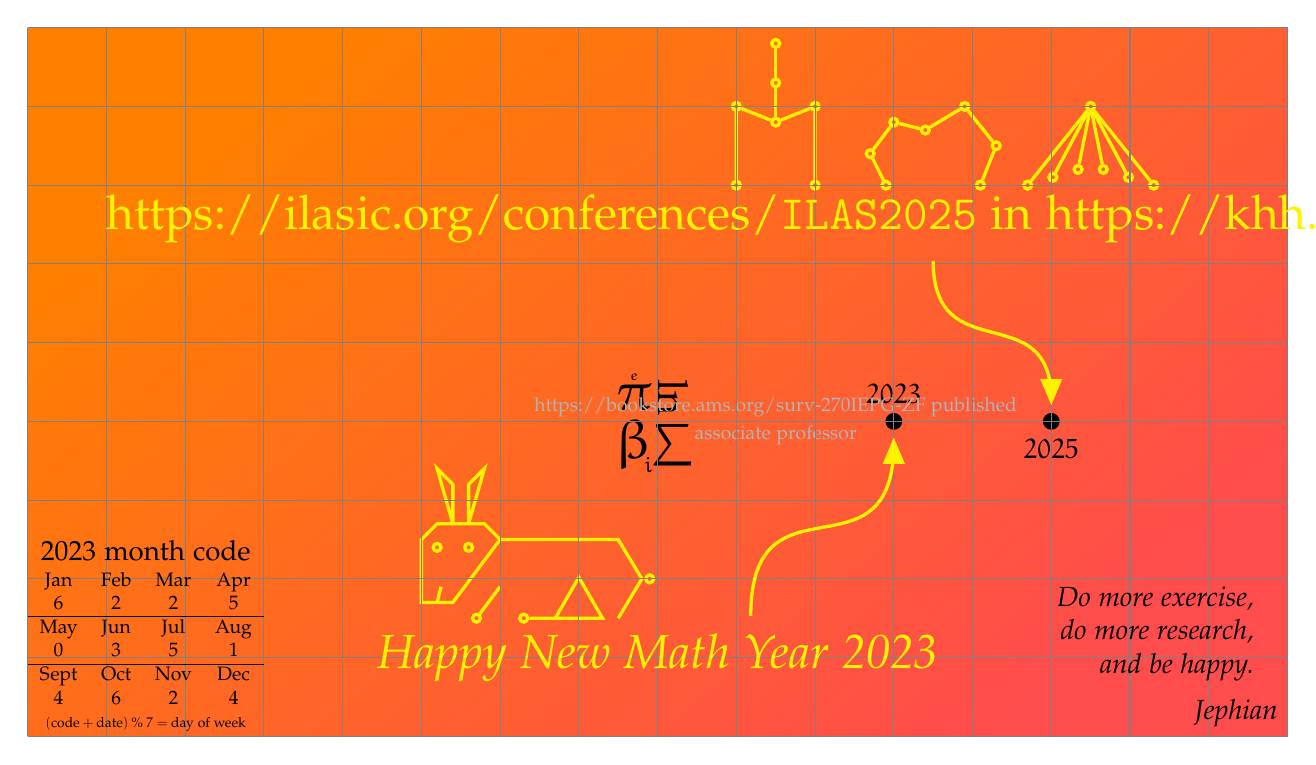
\begin{tikzpicture}
\coordinate (Jamaica) at (-8,-4);
\coordinate (Dominican) at (8,-4);
\coordinate (Cuba) at (-8,5);
\coordinate (TurksCaicos) at (8,5);
\coordinate (Tortuga) at (0,0);
\clip (Jamaica) rectangle (TurksCaicos);

%%Help Lines
\begin{pgfonlayer}{beta}
\draw [step=1, black!50, thin] (Jamaica) grid (TurksCaicos);
%% \draw (0,0) circle [radius=0.2cm];
\end{pgfonlayer}


%%background Layer
\begin{pgfonlayer}{background}
%% \shade [inner color=orange, outer color=red!70] (-8,-4) rectangle (8,5);
%% \shade [left color=orange, right color=red!70] (-8,-4) rectangle (8,5);
%% \shade [inner color=red!30, outer color=blue!30] (-8,-4) rectangle (8,5);
\shade [shading=axis, top color=orange, bottom color=red!70, shading angle=40] (-8,-4) rectangle (8,5);
%% \begin{scope}[opacity=0.2]
%% \foreach \i in {1,2,3,4} {
%%     \pgfmathsetmacro{\ang}{180 - 18 * \i}
%%     \pgfmathsetmacro{\rang}{180 + \ang}
%%     \pic[xshift=-0.5cm, rotate=\rang] at (\ang:3) {totu};
%% }
%% \foreach \i in {1,2,3,4} {
%%     \pgfmathsetmacro{\ang}{270 + 18 * \i}
%%     \pgfmathsetmacro{\rang}{\ang}
%%     \pic[xshift=0.5cm, rotate=\rang] at (\ang:3) {totu};
%% }
%% \end{scope
%% }
\end{pgfonlayer} 


%%Main Layer (main)
\begin{pgfonlayer}{main}

%%% DRAGON
%% https://www.mdbg.net/chinese/dictionary?page=chardict&cdcanoce=0&cdqchi=%E9%BE%8D
\begin{scope}[draw=none, rectangle]
\node[scale=2] (dpi) at (-0.3,0.3) {$\pi$};
\node[yshift=-0.15cm, scale=0.5] (de) at (dpi.north) {$e$};

\node[scale=2] (dbeta) at (-0.3,-0.3) {$\beta$};
\node[xshift=-0.3cm, yshift=0.3cm, scale=0.8] (di) at (dbeta.south east) {$i$};

\node[scale=1.5, rotate=-90] (dln) at (0.2,0.3) {$\ln$};

\node[scale=1.5] (dsigma) at (0.2,-0.3) {$\sum$};
\end{scope}

\node[circle, draw, fill, inner sep=2pt, label={above:$2023$}] (2023) at (3,0) {};
\node[circle, draw, fill, inner sep=2pt, label={below:$2025$}] (2025) at (5,0) {};

%%% KH BUILDINGS
\begin{scope}[yellow, very thick, shift={(3.5,3)}, every node/.style={circle, draw, inner sep=1pt}]

%%% 85 SKY TOWER
\node (851) at (-2.5,0) {};
\node (852) at (-2.5,1) {};
\node (853) at (-1.5,0) {};
\node (854) at (-1.5,1) {};
\node (855) at (-2,0.8) {};
\node (856) at (-2,1.3) {};
\node (857) at (-2,1.8) {};
\draw (851) -- (852) -- (855) -- (854) -- (853);
\draw (855) -- (856) -- (857);

%%% KAOHSIUNG EXHIBITION CENTER
\node (kec1) at (-0.6,0) {};
\node (kec2) at (-0.8,0.4) {};
\node (kec3) at (-0.5,0.8) {};
\node (kec4) at (-0.1,0.7) {};
\node (kec5) at (0.4,1) {};
\node (kec6) at (0.8,0.5) {};
\node (kec7) at (0.6,0) {};
\draw (kec1) -- (kec2) -- (kec3) -- (kec4) -- (kec5) -- (kec6) -- (kec7);

%%% GREAT HABOR BRIDGE
\node (ghb1) at (2,1) {}; 
\node (ghb2) at (1.2,0) {}; 
\node (ghb3) at (1.52,0.1) {}; 
\node (ghb4) at (1.84,0.2) {}; 
\node (ghb5) at (2.16,0.2) {}; 
\node (ghb6) at (2.48,0.1) {}; 
\node (ghb7) at (2.8,0) {}; 
\foreach \i in {2,...,7} {
\draw (ghb1) -- (ghb\i);
}
\end{scope}


%%% RABBIT
\begin{scope}[yellow, very thick, shift={(-1.5,-2.5)}, every node/.style={circle, draw, inner sep=1pt}]

%%% face
\draw (-1.5,1) -- (-1.3,1.2) -- (-0.7,1.2) -- (-0.5,1) -- (-1.1,0.2) -- (-1.5,0.2) -- cycle;
\draw (-1.3,0.2) -- (-1.25,0.4);
%%% ears
\draw (-1.1,1.2) -- ++(0,0.5) -- ++(-0.2,0.2) -- (-1.1,1.2);
\draw (-0.9,1.2) -- ++(0,0.5) -- ++(0.2,0.2) -- (-0.9,1.2);
%%% body
\draw (-0.5,1) -- (1,1) -- (1.3,0.5) -- (1,0);
\node (tail) at (1.4,0.5) {};
%%% legs
\node (leg1) at (-0.8,0) {};
\draw (-0.5,0.4) -- (leg1);
\node (leg2) at (-0.2,0) {};
\draw (leg2) -- (0.8,0) -- ++(120:0.6) -- ++(240:0.6);
%%% eyes
\node (eye1) at (-1.3,0.9) {};
\node (eye2) at (-0.9,0.9) {};
\end{scope}


%%% PROMOTION & BOOK cwp
\node[black!30, above=-2] at (1.5,0) {\scriptsize \href{https://bookstore.ams.org/surv-270}{IEPG-ZF} published};
\node[black!30, below=-2] at (1.5,0) {\scriptsize associate professor};

\end{pgfonlayer}


%%beta layer
\begin{pgfonlayer}{beta}

%%Happy New Math Year
%\draw[decorate,decoration={text along path,text={|\color{red!80!yellow} \LARGE \it|Happy New Math Year 2020}}] (-3.5,-2.5) .. controls (-1,4.5) and (1,4.5) .. (3.5,-2.5);
%% \node[rectangle, draw=none, orange!80!yellow] at (0,-3) {\LARGE\it Happy New Math Year 2023};
\node[rectangle, draw=none, yellow] (hny) at (0,-3) {\LARGE\it Happy New Math Year 2023};
\draw[yellow, very thick, -triangle 45, shorten <=0.1cm, shorten >=0.1cm] (hny.20) .. controls ++(0,2) and ++(0,-2) .. (2023.south);
%% \node[rectangle, draw=none, opacity=0] at (0,-0.5) {\Huge\tt FREE HONG KONG};

%%%ILAS2025
\node[rectangle, draw=none, yellow, below] (ILAS2025) at (3.5,3) {\LARGE \href{https://ilasic.org/conferences/}{\texttt{ILAS2025}} in \href{https://khh.travel/en}{Kaohsiung}!};
\draw[yellow, very thick, -triangle 45, shorten <=0.1cm, shorten >=0.1cm] (ILAS2025.south) .. controls ++(0,-1.5) and ++(0,1.5) .. (2025.north);

%%Month code
\node[above] at (-6.5,-1.9) {2023 month code};
\node[scale=0.7,below] at (-6.5,-1.8) {\begin{tabular}{cccc} 
Jan & Feb & Mar & Apr \\
 6 & 2 & 2 & 5 \\
\hline
May & Jun & Jul & Aug \\
 0 & 3 & 5 & 1 \\
\hline
Sept & Oct & Nov & Dec \\
 4 & 6 & 2 & 4 \\
\end{tabular}};
\node[scale=0.5,above] at (-6.5,-4) {$(\text{code}+\text{date})\mathbin{\%}7=\text{day of week}$};

%%Goal
\node[yshift=1.3cm, xshift=-0.3cm, left, align=right] at (Dominican) {
\it Do more exercise, \\
\it do more research, \\
\it and be happy.};

%%Signature
\node[yshift=0.3cm,left] at (Dominican) {\it Jephian};

\end{pgfonlayer}




\end{tikzpicture}
\end{document}


%%\draw=\path[draw]
%%\clip=\path[clip]
%%\graph=\path[graph]
%%bend right ~ bend right=30 ~ in,out=right30, left 30
%%(left:2)=(180:2)
%%left ~ anchor=east ~ anchor 0
%%for sharp corners: line cap, line joint
%%for elliptical rectangle: smooth circle, plot coordinates, tensions
%For updating 2.10 to 3.0.0
%after moving the folder, it requires 
%sudo texhash 
% to make it work.
%%To convert to jpg: compile the pdf first, and then use the command below
%% convert -density 300 file.pdf -quality 90 file.jpg
%% required to install imagemagick

%% use pdf2png in AUR with Resolution 500 for 2018 
%% use gimp for 2019 (resolution 1890 x 1062, export quality 90)

%% Sample transformation as below
\makeatletter
\def\mytrans{
    \pgfmathparse{\pgf@x+1cm}
    %\pgf@x=\pgfmathresult pt
    \pgfmathsetlength{\pgf@x}{\pgfmathresult pt}
}
\makeatother



